%%%%%%%%%%%%%%%%%%%%%%%%%%%%%%%%%%%%%%%%%%%%%%%%%%%
%
%  New template code for TAMU Theses and Dissertations starting Fall 2012.  
%  For more info about this template or the 
%  TAMU LaTeX User's Group, see http://www.howdy.me/.
%
%  Author: Wendy Lynn Turner 
%	 Version 1.0 
%  Last updated 8/5/2012
%
%%%%%%%%%%%%%%%%%%%%%%%%%%%%%%%%%%%%%%%%%%%%%%%%%%%
%%%                           Section - DSA
%%%%%%%%%%%%%%%%%%%%%%%%%%%%%%%%%%%%%%%%%%%%%%%%%%%
\chapter{\uppercase {Diffusion Synthetic Acceleration for Discontinuous Finite Elements on Unstructured Grids}}
\label{sec::DSA}

%%%%%%%%%%%%%%%%%%%%%%%%%%%%%%%%%%%%%%%%%%%%%%%%%%%
%%%%%%%%%%%%%%%%%%%%%%%%%%%%%%%%%%%%%%%%%%%%%%%%%%%
%%%   Section - Introduction
%%%%%%%%%%%%%%%%%%%%%%%%%%%%%%%%%%%%%%%%%%%%%%%%%%%
%%%%%%%%%%%%%%%%%%%%%%%%%%%%%%%%%%%%%%%%%%%%%%%%%%%
\section{Introduction}
\label{sec::DSA_Introduction}

%%%%%%%%%%%%%%%%%%%%%%%%%%%%%%%%%%%%%%%%%%%%%%%%%%%
%%%%%%%%%%%%%%%%%%%%%%%%%%%%%%%%%%%%%%%%%%%%%%%%%%%
%%%   SubSection - History
\subsection{History}
\label{sec::DSA_Introduction_History}

cleanup the beginning here later...

The ability to efficiently invert the transport (streaming and collision) operator does not necessarily mean that transport solutions can be easily obtained. In general, radiation transport solutions are obtained iteratively. The simplest and widely-used method is a fixed-point scheme ({\em i.e.} richardson iteration) ubiquitously called source iteration (SI) in the transport community. Unfortunately, the iteration process of SI can converge arbitrarily slowly if the problem is optically thick \cite{ref::adams_larsen_iter_methods}. This corresponds to long mean free paths for neutronics problems. This also corresponds to time steps and material heat capacities tending to infinity and zero, respectively, for thermal radiative transport (TRT) problems.

For these problem regimes in which solution is prohibitively slow, additional steps should be taken to speed up, or accelerate, solution convergence \cite{ref::adams_larsen_iter_methods}. The most used methods to assist in solution convergence are often called synthetic acceleration techniques. These techniques were first introduced by Kopp \cite{kopp1963synthetic} and Lebedev \cite{lebedevI,lebedevII,lebedevIII,lebedevIV,lebedevV,lebedevVI,lebedevVII} in the 1960's. From Kopp's and Lebedev's work, Gelbard and Hageman then introduced two synthetic acceleration options for the low-order operator: diffusion and $S_2$ \cite{gelbard1969synthetic}. Their diffusion preconditioning led to efficient convergence properties on fine spatial meshes. Reed then showed that Gelbard and Hageman's diffusion preconditioning would yield a diverging system for coarse meshes \cite{reed1971effectiveness}. At this point in time, no one knew if an unconditionally efficient acceleration method could be derived.

Then in 1976, Alcouffe proposed a remedy to Gelbard and Reed that he called diffusion synthetic acceleration (DSA) \cite{alcouffe1976stable,alcouffe1977DSA,alcouffe1977diffusion}. He showed that if you derived the diffusion operator consistently with the discretized transport operator, then SI could be accelerated with DSA in an efficient and robust manner. Larsen and McCoy then demonstrated that unconditional stability required that consistency be maintained in both spatial and angular discretization in their four-step procedure \cite{larsen1982unconditionally_I,larsen1982unconditionally_II}. However, Adams and Martin then showed that partially-consistent diffusion discretizations could effectively accelerate DFEM discretizations of the neutron transport equation \cite{ref::dsa_DFEM_adams_martin}. Their modified-four-step procedure (M4S), based on Larsen and McCoy's work, was shown to be unconditionally stable for regular geometries, but divergent for unstructured multi-dimensional meshes \cite{warsa2002fully}. In more recent years, alternate discretizations for the diffusion operator have been applied to unstructured multi-dimensional grids. These include the partially consistent Wareing-Larsen-Adams (WLA) DSA \cite{ref::WLA_DSA}, the fully consistent DSA (FCDSA) \cite{warsa2002fully}, and the partially consistent MIP DSA \cite{ref::DSA_wang_ragusa,wang2009adaptive,turcksin2014discontinuous}.

Most recently, the partially consistent MIP DSA method has been shown to be an unconditionally stable acceleration method for the 2D DFEM transport equation on unstructured meshes. Wang showed that it acted as an effective preconditioner for higher-order DFEM discretizations on triangles \cite{ref::DSA_wang_ragusa,wang2009adaptive}. Turcksin and Ragusa then extended the work to arbitrary polygonal meshes \cite{turcksin2014discontinuous}. The MIP diffusion operator is symmetric positive definite (SPD) and was shown to be efficiently invertible with preconditioned conjugate gradient (PCG) and advanced preconditioners such as algebraic multi-grid (AMG) \cite{turcksin2014discontinuous}.

%%%%%%%%%%%%%%%%%%%%%%%%%%%%%%%%%%%%%%%%%%%%%%%%%%%
%%%%%%%%%%%%%%%%%%%%%%%%%%%%%%%%%%%%%%%%%%%%%%%%%%%
%%%   SubSection - Synthetic Acceleration
\subsection{Synthetic Acceleration}
\label{sec::DSA_Introduction_SA}

Synthetic acceleration techniques have been widely used in the nuclear engineering community to improve solution convergence for prohibitively slow problems. We now provide a general framework for how synthetic acceleration methods are derived. We begin by expressing our neutron transport equation in the following form,

\begin{equation}
\label{eq::DSA_simple_trans_eq_w_ops}
\left(  {\bf A} - {\bf B}  \right) \Psi = {\bf Q} ,
\end{equation}

\noindent where ${\bf A}$ and ${\bf B}$ are both linear operators, $\Psi$ is the full angular flux solution in space, angle, and energy, and ${\bf Q}$ is the source or driving function. If we had the ability to efficiently invert $\left(  {\bf A} - {\bf B}  \right)$ directly, then $\Psi$ could be directly computed:

\begin{equation}
\label{eq::DSA_simple_trans_eq_w_ops_inverted}
\Psi = \left(  {\bf A} - {\bf B}  \right)^{-1} {\bf Q} .
\end{equation}

\noindent However, since in practice the discretized version of $\left(  {\bf A} - {\bf B}  \right)$ is much more costly to directly invert than the discretized version of ${\bf A}$, we instead choose to iteratively solve for $\Psi$.

To compute $\Psi$, the following iterative system of equations is usually employed,

\begin{equation}
\label{eq::DSA_simple_trans_eq_w_ops_iterates}
 {\bf A} \Psi^{(k+1)} - {\bf B}  \Psi^{(k)} = {\bf Q} ,
\end{equation}

\noindent where directly solving for $\Psi^{(k+1)}$ yields the following:

\begin{equation}
\label{eq::DSA_simple_trans_eq_sol_w_ops_iterates}
 \Psi^{(k+1)} =  {\bf A}^{-1} {\bf B}  \Psi^{(k)} +  {\bf A}^{-1} {\bf Q} .
\end{equation}

\noindent For brevity, we define a new operator ${\bf C} = {\bf A}^{-1} {\bf B}$ which is known as the iteration operator. The spectral radius, $\rho$, of this operator is simply the supremum of the absolute values of its eigenvalues. For this work, we assume that $\rho$ is less than unity to guarantee convergence. We next define the residual, $r^{(k)}$, as the difference between two successive solution iterates,

\begin{equation}
\label{eq::DSA_synthetic_eq_residual}
r^{(k)} = \Psi^{(k)} - \Psi^{(k-1)} ,
\end{equation}

\noindent which can also be written as the following:

\begin{equation}
\label{eq::DSA_synthetic_eq_residual_op}
r^{(k)} = {\bf C}\Psi^{(k-1)} .
\end{equation}

With the iteration operator, ${\bf C}$, and the residual for iterate $k$ , $r^{(k)}$, defined, we can then write the true, converged solution in terms of the solution at iteration $k$ and an infinite series of residuals:

\begin{equation}
\label{eq::DSA_synthetic_eq_true_sol}
\Psi = \Psi^{(k)} + \sum_{n=1}^{\infty} r^{(k+n)} .
\end{equation}

\noindent Using both Eqs. (\ref{eq::DSA_synthetic_eq_residual_op}) and (\ref{eq::DSA_synthetic_eq_true_sol}), we can rewrite Eq. (\ref{eq::DSA_synthetic_eq_true_sol}) using the iteration operator and the last residual,

\begin{equation}
\label{eq::DSA_synthetic_eq_true_sol_it_op}
\Psi = \Psi^{(k)} + \left(  {\bf I} + {\bf C} + {\bf C}^2 + ...  \right) {\bf C} r^{(k)}.
\end{equation}

\noindent Since we have assumed that the spectral radius of {\bf C} is less than unity, the infinite operator series of Eq. (\ref{eq::DSA_synthetic_eq_true_sol_it_op}) converges to $\left(  {\bf I} - {\bf C}   \right)^{-1} {\bf C}$. This means that we can succinctly write Eq. (\ref{eq::DSA_synthetic_eq_true_sol_it_op}) as the following:

\begin{equation}
\label{eq::DSA_synthetic_eq_true_sol_it_op_succinct}
\Psi = \Psi^{(k)} + \left(  {\bf I} - {\bf C}   \right)^{-1} {\bf C} r^{(k)}.
\end{equation}

\noindent By using the definition of ${\bf C}$ along with some linear algebra, Eq. (\ref{eq::DSA_synthetic_eq_true_sol_it_op_succinct}) becomes 

\begin{equation}
\label{eq::DSA_synthetic_eq_true_sol_orig_ops}
\Psi = \Psi^{(k)} + \left(  {\bf A} - {\bf B}   \right)^{-1} {\bf B} r^{(k)}.
\end{equation}

We would like to use the results of Eq. (\ref{eq::DSA_synthetic_eq_true_sol_orig_ops}) to immediately compute our exact transport solution, $\Psi$. However, this would require the inversion of $\left(  {\bf A} - {\bf B}  \right)$ which we did not employ originally in Eq. (\ref{eq::DSA_simple_trans_eq_w_ops}) because of the difficulty. This means that, in its current form, Eq. (\ref{eq::DSA_synthetic_eq_true_sol_orig_ops}) is no more useful to us than Eq. (\ref{eq::DSA_simple_trans_eq_w_ops}). This would then be an exercise in futility if we were restricted to only working with the $\left(  {\bf A} - {\bf B}  \right)$ operator. Instead, suppose that we could define an operator, ${\bf W}$, that closely approximates $\left(  {\bf A} - {\bf B}  \right)$ but it is easily invertible. If ${\bf W}$ efficiently approximates the slowest converging error modes of $\left(  {\bf A} - {\bf B}  \right)$, then Eq. (\ref{eq::DSA_synthetic_eq_true_sol_orig_ops}) can be modified to form a new iterative procedure.

The new iterative procedure begins by simply taking the half-iterate of Eq. (\ref{eq::DSA_simple_trans_eq_sol_w_ops_iterates}) instead of its full version: ${(k+1/2)}$ instead of {(k+1)}. This half-iterate has the form

\begin{equation}
\label{eq::DSA_synthetic_eq_half_it}
\Psi^{(k+1/2)} = {\bf C} \Psi^{(k)} + {\bf A}^{-1} {\bf Q}.
\end{equation}

\noindent We can then express the full-iterate by the suggestion of Eq. (\ref{eq::DSA_synthetic_eq_true_sol_orig_ops}). Using the low-order operator, we express the full-iterate as the following,

\begin{equation}
\label{eq::DSA_synthetic_eq_half_it_correction}
\Psi^{(k+1)} =\Psi^{(k+1/2)} + {\bf W}^{-1} {\bf B}  r^{(k+1/2)},
\end{equation}

\noindent where $r^{(k+1/2)} = \Psi^{(k+1/2)} - \Psi^{(k)}$. We can also express Eq. (\ref{eq::DSA_synthetic_eq_half_it_correction}) in terms of just the previous iterate ,$\Psi^{(k)}$, and a new operator:

\begin{equation}
\label{eq::DSA_synthetic_eq_new_algo}
\Psi^{(k+1)} = \left[  {\bf I} - {\bf W}^{-1} \left(  {\bf A} - {\bf B}  \right)  \right] {\bf C} \Psi^{(k)} + \left({\bf I} + {\bf W}^{-1} {\bf B} \right) {\bf A}^{-1} {\bf Q} .
\end{equation}

\noindent Observe that as ${\bf W}$ more closely approximates $\left(  {\bf A} - {\bf B}  \right)$, the operator ${\bf W}^{-1} \left(  {\bf A} - {\bf B}  \right)$ converges to the identity matrix, ${\bf I}$. This means that the spectral radius of this new iteration matrix will approach zero as ${\bf W}$ gets closer to $\left(  {\bf A} - {\bf B}  \right)$ and therefore more quickly and efficiently converge to the true solution.

%%%%%%%%%%%%%%%%%%%%%%%%%%%%%%%%%%%%%%%%%%%%%%%%%%%
%%%%%%%%%%%%%%%%%%%%%%%%%%%%%%%%%%%%%%%%%%%%%%%%%%%
%%%   Section - DSA
%%%%%%%%%%%%%%%%%%%%%%%%%%%%%%%%%%%%%%%%%%%%%%%%%%%
%%%%%%%%%%%%%%%%%%%%%%%%%%%%%%%%%%%%%%%%%%%%%%%%%%%
\section{Diffusion Synthetic Acceleration Methodologies}
\label{sec::DSA_DSA}

The procedures outlined in Section \ref{sec::DSA_Introduction_SA} define a general methodology to perform synthetic acceleration on the transport equation. We could utilize any of the acceleration strategies that have been developed over the years including DSA, TSA, BPA, etc. The only difference arises in what form the low-order operator, ${\bf W}$, will take. We obviously are focusing on DSA for this dissertation work, and we do so by first describing in Section \ref{sec::DSA_DSA_1G} a simple 1-group specification of the synthetic acceleration methodology just presented. We then present a pair of strategies that can be employed to accelerate thermal neutron upscattering in Section \ref{sec::DSA_DSA_MG}.

%%%%%%%%%%%%%%%%%%%%%%%%%%%%%%%%%%%%%%%%%%%%%%%%%%%
%%%%%%%%%%%%%%%%%%%%%%%%%%%%%%%%%%%%%%%%%%%%%%%%%%%
%%%   SubSection - 1-group
\subsection{Simple 1-group DSA Strategy}
\label{sec::DSA_DSA_1G}

\begin{equation}
\label{eq::DSA_simple_trans_eq}
\vec{\Omega} \cdot \vec{\nabla} \psi_m + \sigma_t \psi_m = \frac{\sigma_s}{4 \pi} \phi + \frac{Q}{4 \pi}, \qquad m=1,...,M
\end{equation}

\begin{equation}
\label{eq::DSA_simple_trans_eq_it}
\left[ \vec{\Omega} \cdot \vec{\nabla} + \sigma_t \right] \psi_m^{(k+1/2)} = \frac{\sigma_s}{4 \pi} \phi^{(k)} + \frac{Q}{4 \pi}, \qquad m=1,...,M
\end{equation}

%%%%%%%%%%%%%%%%%%%%%%%%%%%%%%%%%%%%%%%%%%%%%%%%%%%
%%%%%%%%%%%%%%%%%%%%%%%%%%%%%%%%%%%%%%%%%%%%%%%%%%%
%%%   SubSection - MG
\subsection{DSA Acceleration Strategies for Thermal Neutron Upscattering}
\label{sec::DSA_DSA_MG}

%%%%%%%%%%%%%
%%%   SubSubSection - Two-Grid
\subsubsection{Multigroup Richardson Acceleration}
\label{sec:DSA_DSA_MG_WGS}

\begin{equation}
\label{eq::DSA_WG_trans_it_eq}
{\bf L_{gg}} \psi_g^{(k+1/2)} =  {\bf M} \sum_{g'=1}^G {\bf \Sigma}_{g g'} \phi_{g'}^{(k)} + {\bf Q}_g
\end{equation}


%%%%%%%%%%%%%
%%%   SubSubSection - Two-Grid
\subsubsection{Two-Grid Acceleration}
\label{sec:DSA_DSA_MG_TG}

The second acceleration methodology that we will investigate is the two-grid acceleration scheme devised by Adams and Morel \cite{adams1993two}. The derived the 

\begin{equation}
\label{eq::DSA_TG_trans_it_eq}
{\bf L_{gg}} \psi_g^{(k+1/2)} = {\bf M} \sum_{g'=1}^g {\bf \Sigma}_{g g'} \phi_{g'}^{(k+1/2)} + {\bf M} \sum_{g'=g+1}^G {\bf \Sigma}_{g g'} \phi_{g'}^{(k)} + {\bf Q}_g
\end{equation}

\noindent In operator form, the full solution and half-iterate equations are given by

\begin{equation}
\label{eq::DSA_TG_trans_eq_ops}
{\bf L} \Psi = {\bf M} {\bf S_D} \Phi + {\bf M} {\bf S_U} \Phi + {\bf Q} ,
\end{equation}

\noindent and

\begin{equation}
\label{eq::DSA_TG_trans_it_eq_ops}
{\bf L} \Psi^{(k+1/2)} = {\bf M} {\bf S_D} \Phi^{(k+1/2)} + {\bf M} {\bf S_U} \Phi^{(k)} + {\bf Q} ,
\end{equation}

\noindent respectively. ${\bf S_D}$ and ${\bf S_U}$ are the downscatter and upscatter portions of the scattering matrix, respectively. These matrices still contain all of the scattering moments; they are simply restricted in energy. By moving the downscattering portion to the left side of the equation, inverting the ${\bf L}$ operator, and applying the discrete-to-moment operator, ${\bf D}$, we can rewrite the iteration equation of Eq. (\ref{eq::DSA_TG_trans_it_eq_ops}) in terms of only the flux moments:

\begin{equation}
\label{eq::DSA_TG_half_it}
\left[ {\bf I} - {\bf D}{\bf L}^{-1} {\bf M} {\bf S_D} \right]\Phi^{(k+1/2)} = {\bf D}{\bf L}^{-1}  {\bf M} {\bf S_U} \Phi^{(k)} + {\bf D}{\bf L}^{-1}  {\bf Q}
\end{equation}

\noindent By inverting the left-side operator, we directly solve for the half-iterate flux moments,

\begin{equation}
\label{eq::DSA_TG_half_it_sol}
\begin{aligned}
\Phi^{(k+1/2)} &= \left[ {\bf I} - {\bf D}{\bf L}^{-1} {\bf M} {\bf S_D} \right]^{-1} {\bf D}{\bf L}^{-1}  {\bf M} {\bf S_U} \Phi^{(k)} + {\bf b}  \\
{\bf b} &= \left[ {\bf I} - {\bf D}{\bf L}^{-1} {\bf M} {\bf S_D} \right]^{-1} {\bf D}{\bf L}^{-1}  {\bf Q}
\end{aligned} ,
\end{equation}

\noindent where we reduced the driving function to ${\bf b}$ for brevity.

%%%%%%%%%%%%%%%%%%%%%%%%%%%%%%%%%%%%%%%%%%%%%%%%%%%
%%%%%%%%%%%%%%%%%%%%%%%%%%%%%%%%%%%%%%%%%%%%%%%%%%%
%%%   Section - SIP
%%%%%%%%%%%%%%%%%%%%%%%%%%%%%%%%%%%%%%%%%%%%%%%%%%%
%%%%%%%%%%%%%%%%%%%%%%%%%%%%%%%%%%%%%%%%%%%%%%%%%%%
\section{Symmetric Interior Penalty Form of the Diffusion Equation}
\label{sec::DSA_SIP}

So far, we have presented several strategies in Section \ref{sec::DSA_DSA} in which DSA can be used to accelerate both within-group scattering and upscattering. We have also simply stated that our low-order operator will be the diffusion equation. However, we have not presented the exact form of the diffusion equation that we will utilize. In Section \ref{sec::DSA_MIP}, we present the full form of the modified interior penalty (MIP) form of the diffusion equation that we will use as our low-order operator for DSA calculations. However, we first present in this Section a more generalized version of the interior penalty form that we could use as a stand-alone solver for the standard diffusion equation: the symmetric interior penalty (SIP) form \cite{arnold2002unified,ragusa2015discontinuous,ref::SIP_3D}.

We begin our discussion of the SIP form by analyzing the standard form of the diffusion equation,

\begin{equation}
\label{eq::DSA_standard_diff_eq}
- \vec{\nabla}  \cdot D (\vec{r})  \vec{\nabla} \Phi (\vec{r}) + \sigma \Phi (\vec{r}) = Q (\vec{r}) , \qquad \vec{r} \in \mathcal{D} ,
\end{equation}

\noindent with Dirichlet boundary conditions

\begin{equation}
\label{eq::DSA_standard_diff_eq_dirichlet_bound}
\Phi (\vec{r}) = \Phi_0 (\vec{r}), \qquad \vec{r} \in \partial \mathcal{D}^d ,
\end{equation}

\noindent Neumann boundary conditions

\begin{equation}
\label{eq::DSA_standard_diff_eq_neumann_bound}
- D \partial_n \Phi (\vec{r}) = J_0 (\vec{r}), \qquad \vec{r} \in \partial \mathcal{D}^n ,
\end{equation}

\noindent and Robin boundary conditions

\begin{equation}
\label{eq::DSA_standard_diff_eq_robin_bound}
\frac{1}{4}\Phi (\vec{r}) + \frac{D}{2} \partial_n \Phi (\vec{r}) = J^{inc} (\vec{r}), \qquad \vec{r} \in \partial \mathcal{D}^r .
\end{equation}



\begin{equation}
\label{eq::penalty_boundary_term}
\Phi (\vec{r}) +\frac{1}{\kappa} D \partial_n \Phi (\vec{r}) = \Phi_0 (\vec{r}), \qquad \vec{r} \in \partial \mathcal{D}^d, \qquad \kappa \gg 1
\end{equation}

\begin{equation}
\label{eq::SIP_boundary_laplacian_term}
\begin{aligned}
\Big<  D \vec{\nabla}  \Phi , \vec{\nabla} \Phi^*  \Big>_{\mathcal{D}} - \Big\{   D \partial_n \Phi, \Phi^* \Big\}_{\partial \mathcal{D}^d} - \Big\{  \Phi, D \partial_n \Phi^* \Big\}_{\partial \mathcal{D}^d} \\ + \Big\{ \kappa (\Phi - \Phi_0),  \Phi^* \Big\}_{\partial \mathcal{D}^d} = - \Big\{  \Phi_0, D \partial_n \Phi^* \Big\}_{\partial \mathcal{D}^d} 
\end{aligned}
\end{equation}

\begin{equation}
\label{eq::SIP_interior_laplacian_term}
\Big\{ \kappa [\![   \Phi ]\!] , [\![  \Phi^* ]\!]\Big\}_{E_h^i} + \Big\{  [\![   \Phi ]\!] , \{\!\{  D \partial_n \Phi^* \}\!\}\Big\}_{E_h^i} + \Big\{ \{\!\{  D \partial_n  \Phi \}\!\} , [\![  \Phi^* ]\!]\Big\}_{E_h^i} = 0
\end{equation}

The mean value and the jump of the terms on a face are

\begin{equation}
\label{eq::solution_mean_and_jump}
\{\!\{  \Phi \}\!\} \equiv \frac{\Phi^+ + \Phi^-}{2} \qquad \text{and} \qquad [\![   \Phi ]\!] \equiv \Phi^+ - \Phi^- ,
\end{equation}

\noindent respectively. The directionality of the terms across a face can be defined in negative, $\Phi^-$, and positive, $\Phi^+$ directions by their trace:

\begin{equation}
\label{eq::solution_trace}
\Phi^{\pm} \equiv \lim_{s \rightarrow 0^{\pm}} \Phi (\vec{r} + s \vec{n}),
\end{equation}

\noindent where the face's unit normal direction, $\vec{n}$, has been ar

Using Eqs. (\ref{eq::SIP_boundary_laplacian_term}) and (\ref{eq::SIP_interior_laplacian_term}), the SIP form of the diffusion equation can be succinctly written as

\begin{equation}
a^{SIP}( \Phi, \Phi^*) = b^{SIP}(\Phi^*),
\label{eq::SIP_weak_form}
\end{equation}

\noindent with the following bilinear matrix:

\begin{equation}
\label{eq::SIP_bilinear_form}
\begin{aligned}
a^{SIP}( \Phi, \Phi^*)  = \Big<  D \vec{\nabla}  \Phi , \vec{\nabla} \Phi^*  \Big>_{\mathcal{D}} + \Big<  \sigma   \Phi ,  \Phi^*  \Big>_{\mathcal{D}}  +  \frac{1}{2} \Big\{    \Phi , \Phi^* \Big\}_{\partial \mathcal{D}^r}   \\
+  \Big\{ \kappa_e^{SIP} [\![   \Phi ]\!] , [\![  \Phi^* ]\!]\Big\}_{E_h^i} + \Big\{  [\![   \Phi ]\!] , \{\!\{  D \partial_n \Phi^* \}\!\}\Big\}_{E_h^i}  + \Big\{ \{\!\{  D \partial_n  \Phi \}\!\} , [\![ \Phi^* ]\!]\Big\}_{E_h^i} \\
+ \Big\{ \kappa_e^{SIP}   \Phi ,   \Phi^* \Big\}_{\partial \mathcal{D}^d} - \Big\{   \Phi  ,  D \partial_n \Phi^* \Big\}_{\partial \mathcal{D}^d} - \Big\{   D 				\partial_n  \Phi , \Phi^* \Big\}_{\partial \mathcal{D}^d}  
\end{aligned} ,
\end{equation}

\noindent and with the following linear right-hand-side:

\begin{equation}
\label{eq::SIP_linear_form}
\begin{aligned}
b^{SIP} (\Phi^*) = \Big<  Q, \Phi^*  \Big>_{\mathcal{D}}  - \Big\{   J_{0}, \Phi^*  \Big\}_{\partial \mathcal{D}^n} +  2 \Big\{   J^{inc}, \Phi^*  \Big\}_{\partial 				\mathcal{D}^r} \\ + \Big\{ \kappa_e^{SIP}   \Phi_0 ,   \Phi^* \Big\}_{\partial \mathcal{D}^d} - \Big\{   \Phi_0  ,  D \partial_n \Phi^* \Big\}_{\partial 					\mathcal{D}^d} 
\end{aligned} .
\end{equation}

\noindent As previously stated, the general penalty term, $\kappa$ of Eqs. (\ref{eq::penalty_boundary_term} - \ref{eq::SIP_interior_laplacian_term}) needs to have sufficient positive measure to ensure stability. From previous investigations \cite{ref::DSA_2D_arb_poly,wang2009adaptive,ref::DSA_wang_ragusa}, we choose the penalty coefficient to be face dependent:

\begin{equation}
\kappa_e^{SIP} = 
\begin{cases}
	\frac{c}{2} \left(  \frac{D^+}{h^+} + \frac{D^-}{h^-} \right) & e \in E_h^i\\ 
	c \frac{D^-}{h^-}& e \in \partial \mathcal{D}
\end{cases},
\label{eq::SIP_penalty_term}
\end{equation}

\noindent for interior, $E_h^i$, and boundary, $\partial \mathcal{D}$, faces respectively. In Eq. (\ref{eq::SIP_penalty_term}), $h^\pm$ is the orthogonal projection of the face, $e$, into the cells defined by the trace in Eq. (\ref{eq::solution_trace}). Turcksin and Ragusa, \cite{turcksin2014discontinuous}, defined $h^\pm$ for 2D polygons, whose definitions can be seen in Table \ref{tab::orth_proj_2D}. The orthogonal projection for both triangles and quadrilaterals can be explicitly defined from simple geometric relationships. However, for polygons with $>4$ faces, there is no explicit geometric relationship to define the orthogonal projection. Instead, the polygon is approximated as regular, and the orthogonal projection is no longer face-dependent. For polygons with an even number of faces greater than 4, the orthogonal projection is twice the apothem, which is the line segment between the polygon's center and the midpoint of each polygon's side. For odd number of faces greater than 4, the polygon's orthogonal projection becomes the sum of the apothem and the circumradius.

 In a similar manner to the 2D orthogonal projections defined in Table \ref{tab::orth_proj_2D}, we define our choice for the extension of the orthogonal projections to 3D in Table \ref{tab::orth_proj_3D}. Like triangles and quadrilaterals in 2D, the orthogonal projections for tetrahedra and hexahedra can be explicitly defined from the volume equations for pyramids and parallelepipeds, respectively. For cells that are not tetrahedra or hexahedra, we introduce an approximation similar to 2D where we treat the cell as a regular polyhedron. In 3D there is no compact formula that can be given, unlike the definitions of the apothem and circumradius for 2D. Instead, we take the geometric limit of a polyhedra as the number of faces tends to infinity (a sphere). In this limiting case, the orthogonal projection simply becomes the sphere's diameter. We can then define the sphere's diameter with geometric information that would also be available to polyhedra by dividing a sphere's volume (the polyhedral volume) by its surface area (the sum of the areas of the polyhedral faces). While this leads to a gross approximation of the orthogonal projection for polyhedra that are not tetrahedra or hexahedra, it will provide appropriate geometric measure, especially for strictly convex polyhedra.

\begin{table}[h]
\centering
\caption{Orthogonal projection, $h$, for different polygonal types: $A_K$ is the area of cell $K$, $L_e$ is the length of face $e$, and $P_K$ is the perimeter of cell $K$.}
\def\arraystretch{1.4}
\begin{tabular}{|c|c|c|c|c|}
	\hline
	Number of Vertices & 3 & 4 & $>4$ and even& $>4$ and odd \\
	\hline
	$h$ & $2 \frac{A_K}{L_e}$ & $\frac{A_K}{L_e}$ & $4 \frac{A_K}{P_K}$ & $2 \frac{A_K}{P_K} + \sqrt{\frac{2 A_K}{N_K \sin(\frac{2 \pi}{N_K})}}$ \\
	\hline
\end{tabular}
\label{tab::orth_proj_2D}
\end{table}



\begin{table}[h]
\centering
\caption{Orthogonal projection, $h$, for different polyhedral types: $V_K$ is the volume of cell $K$, $A_e$ is the area of face $e$, and $SA_K$ is the surface area of cell $K$.}
\def\arraystretch{1.4}
\begin{tabular}{|c|c|c|c|}
	\hline
	Number of Faces & 4 & 6 & otherwise \\
	\hline
	$h$ & $3 \frac{V_K}{A_e}$ & $\frac{V_K}{A_e}$ & $6 \frac{V_K}{SA_K}$  \\ [1ex]
	\hline
\end{tabular}
\label{tab::orth_proj_3D}
\end{table}

%%%%%%%%%%%%%%%%%%%%%%%%%%%%%%%%%%%%%%%%%%%%%%%%%%%
%%%%%%%%%%%%%%%%%%%%%%%%%%%%%%%%%%%%%%%%%%%%%%%%%%%
%%%   Section - MIP
%%%%%%%%%%%%%%%%%%%%%%%%%%%%%%%%%%%%%%%%%%%%%%%%%%%
%%%%%%%%%%%%%%%%%%%%%%%%%%%%%%%%%%%%%%%%%%%%%%%%%%%
\section{Modified Interior Penalty Form of the Diffusion Equation used for Diffusion Synthetic Acceleration Applications}
\label{sec::DSA_MIP}

\begin{equation}
a^{MIP}( \delta \Phi, \Phi^*) = b^{MIP}(\Phi^*),
\label{eq::MIP_weak_form}
\end{equation}

\noindent with the following bilinear matrix:

\begin{equation}
\label{eq::MIP_bilinear_form}
\begin{aligned}
a^{MIP}(\delta \Phi, \Phi^*)  = \Big<  D \vec{\nabla} \delta  \Phi , \vec{\nabla} \Phi^*  \Big>_{\mathcal{D}} + \Big<  \sigma \delta  \Phi ,  \Phi^*  \Big>_{\mathcal{D}}    \\
+  \Big\{ \kappa_e^{MIP} [\![ \delta  \Phi ]\!] , [\![  \Phi^* ]\!]\Big\}_{E_h^i} + \Big\{  [\![  \delta \Phi ]\!] , \{\!\{  D \partial_n \Phi^* \}\!\}\Big\}_{E_h^i}  + \Big\{ \{\!\{  D \partial_n \delta \Phi \}\!\} , [\![ \Phi^* ]\!]\Big\}_{E_h^i} \\
+ \Big\{ \kappa_e^{MIP}  \delta \Phi ,   \Phi^* \Big\}_{\partial \mathcal{D}^d} - \frac{1}{2} \Big\{  \delta \Phi  ,  D \partial_n \Phi^* \Big\}_{\partial \mathcal{D}^d} - \frac{1}{2} \Big\{   D \partial_n \delta  \Phi , \Phi^* \Big\}_{\partial \mathcal{D}^d}  
\end{aligned} ,
\end{equation}

\noindent and with the following linear right-hand-side:

\begin{equation}
\label{eq::MIP_linear_form}
b^{MIP} (\Phi^*) = \Big<  Q, \Phi^*  \Big>_{\mathcal{D}}  + \Big\{ \delta  J^{inc}, \Phi^*  \Big\}_{\partial \mathcal{D}^r} .
\end{equation}



\begin{figure}
\label{fig::IP_cart_tri_meshes}
\centering
	\begin{subfigure}[b]{0.48\textwidth}
		\centering
		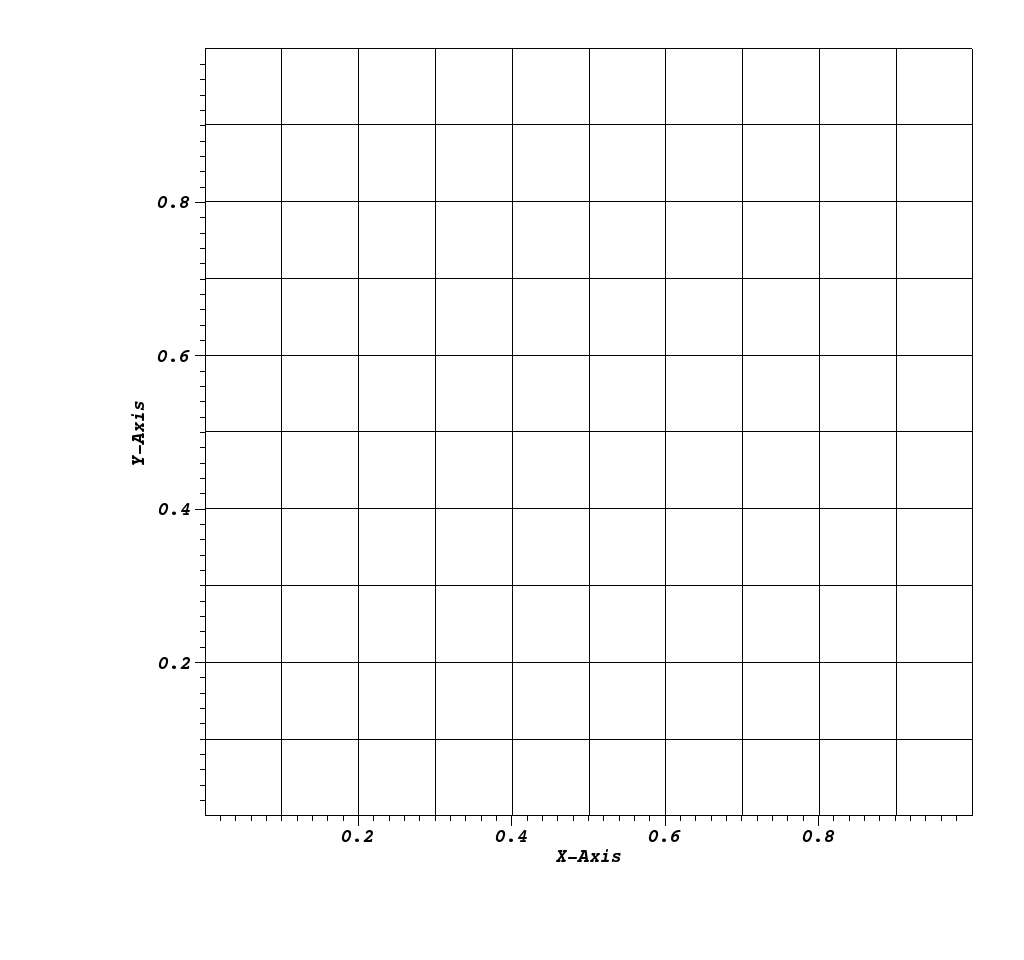
\includegraphics[width=\textwidth]{figures/sec_DSA/IP_cart_mesh.png}
		\caption{}
	\end{subfigure}
	\hfill
	\begin{subfigure}[b]{0.48\textwidth}
		\centering
		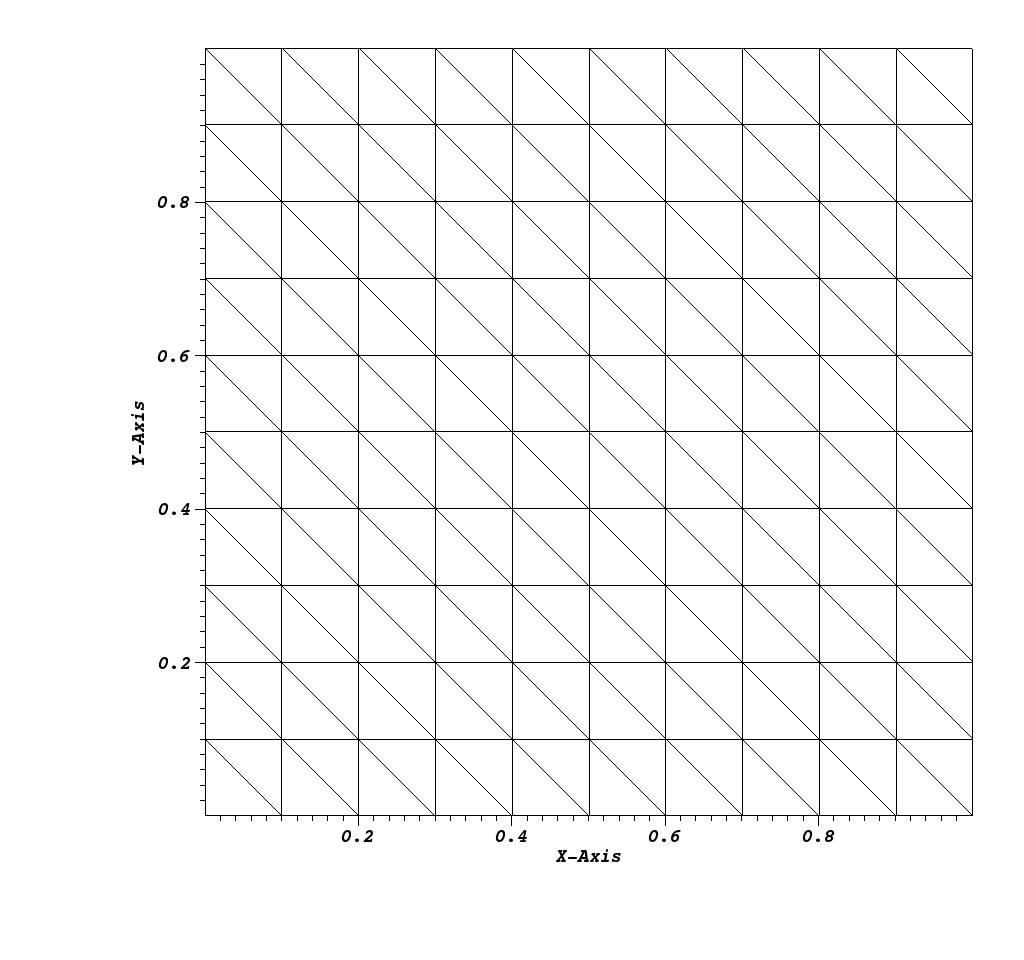
\includegraphics[width=\textwidth]{figures/sec_DSA/IP_tri_mesh.png}
		\caption{}
	\end{subfigure}
\caption{blah}
\end{figure}

\begin{figure}
\centering
\label{fig::IP_coefficient_degradation}
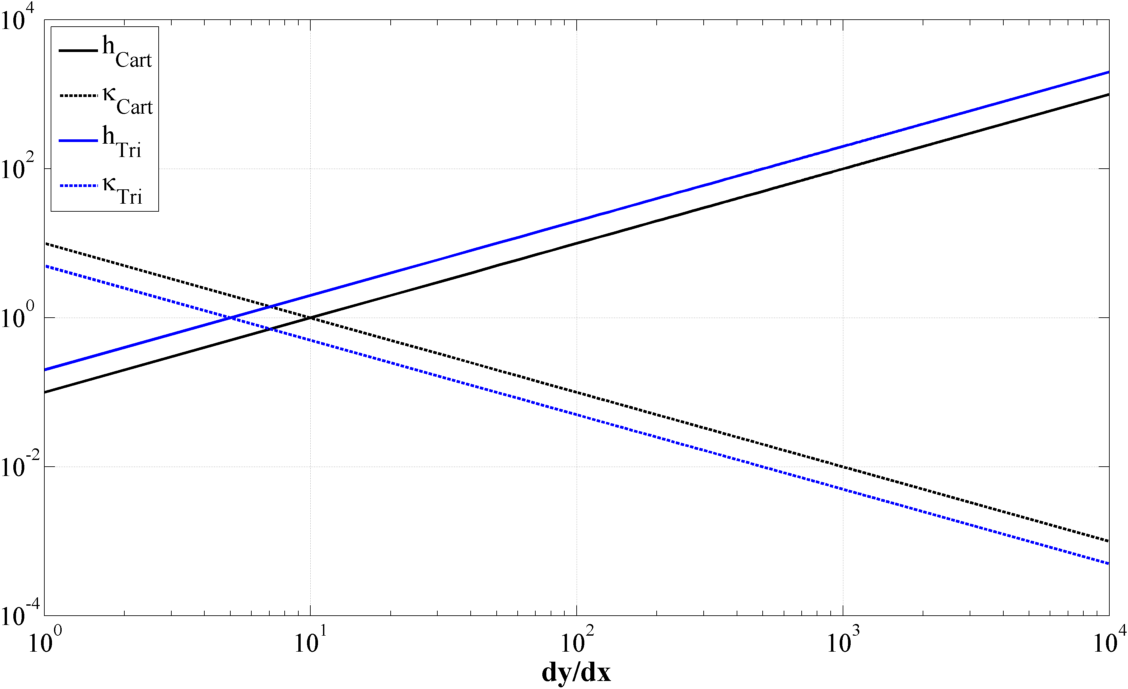
\includegraphics[width=0.8\textwidth]{figures/sec_DSA/IP_penalty_coeff.png}
\caption{Maximum SIP orthogonal projections (solid) and penalty coefficients (dashed) on ordered cartesian (black) and triangular (blue) grids. }
\end{figure}

\begin{equation}
\label{eq::MIP_penalty_term}
\kappa_e^{MIP} = \text{max} \left( \kappa_e^{SIP}, \frac{1}{4} \right)
\end{equation}

%%%%%%%%%%%%%%%%%%%%%%%%%%%%%%%%%%%%%%%%%%%%%%%%%%%
%%%%%%%%%%%%%%%%%%%%%%%%%%%%%%%%%%%%%%%%%%%%%%%%%%%
%%%   Section - Fourier
%%%%%%%%%%%%%%%%%%%%%%%%%%%%%%%%%%%%%%%%%%%%%%%%%%%
%%%%%%%%%%%%%%%%%%%%%%%%%%%%%%%%%%%%%%%%%%%%%%%%%%%
\section{Fourier Analysis}
\label{sec::DSA_Fourier}

\begin{figure}
\centering
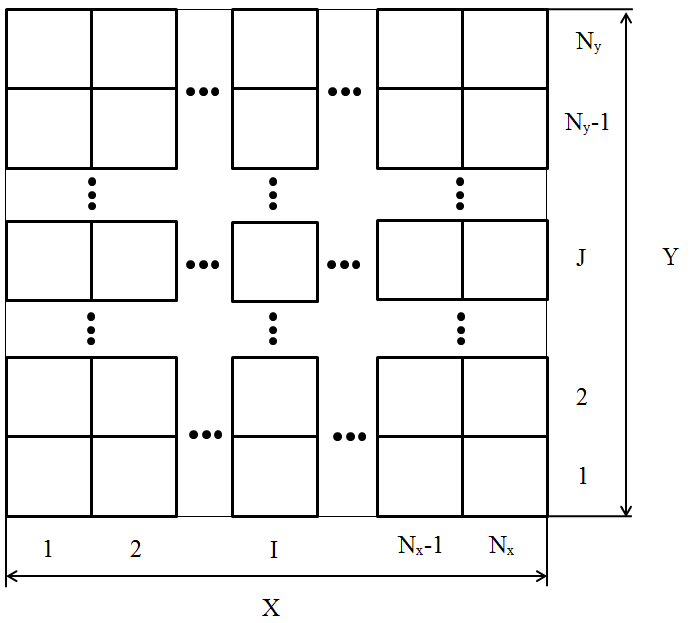
\includegraphics[width=0.60\textwidth]{figures/sec_DSA/fourier_sq_layout.png}
\caption{Fourier domain for 2D quadrilateral cells or an axial slice of 3D hexahedral cells in a regular grid.}
\label{fig::}
\end{figure}

\begin{equation}
\label{eq::fourier_sol}
\begin{aligned}
\Psi_m (\vec{r}) = \hat{\Psi}_m e^{i \vec{\lambda} \cdot \vec{r}}\\
\Phi (\vec{r}) = \hat{\Phi} e^{i \vec{\lambda} \cdot \vec{r}}
\end{aligned}
\end{equation}

\noindent where $i=\sqrt{-1}$

%%%%%%%%%%%%%%%%%%%%%%%%%%%%%%%%%%%%%%%%%%%%%%%%%%%
%%%%%%%%%%%%%%%%%%%%%%%%%%%%%%%%%%%%%%%%%%%%%%%%%%%
%%%   Section - Results
%%%%%%%%%%%%%%%%%%%%%%%%%%%%%%%%%%%%%%%%%%%%%%%%%%%
%%%%%%%%%%%%%%%%%%%%%%%%%%%%%%%%%%%%%%%%%%%%%%%%%%%
\section{Numerical Results}
\label{sec::DSA_Results}

We now present the results showing the efficacy of a discontinuous diffusion form which can be used as a DSA preconditioner for the transport equation discretized over arbitrary grids. We first present the SIP form and how it performs as a pure diffusion solver on unstructured polyhedral grids in Section \ref{sec::DSA_Results_SIP}. We next present the theoretical performance limits of the MIP form as a DSA preconditioner using Fourier Analysis in Section \ref{sec::DSA_Results_Fourier}. We finish by presenting the results of MIP's use as a DSA preconditioner for several different problem types in Section \ref{sec::DSA_Results_MIP}.

%%%%%%%%%%%%%%%%%%%%%%%%%%%%%%%%%%%%%%%%%%%%%%%%%%%
%%%%%%%%%%%%%%%%%%%%%%%%%%%%%%%%%%%%%%%%%%%%%%%%%%%
%%%   SubSection - Thick Diffusive Limit
\subsection{Transport Solutions in the Thick Diffusive Limit}
\label{sec::DSA_Results_TDL}

We present our first numerical example by demonstrating that the various polygonal finite element basis sets satisfy the thick diffusion limit. 


\begin{equation}
\label{eq::BF_Results_TDL_scaling}
\begin{aligned}
	\sigma_t &\rightarrow \frac{\sigma_t}{\epsilon} \\
	\sigma_a &\rightarrow \epsilon \sigma_t\\
	\frac{Q_0}{4 \pi} &\rightarrow \epsilon \frac{Q_0}{4 \pi}
\end{aligned}
\end{equation}

\begin{equation}
\label{eq::BF_Results_TDL_scaled_trans_eq}
\vec{\Omega} \cdot \vec{\nabla} \Psi + \frac{\sigma_t}{\epsilon} \Psi = \sigma_t \left( \frac{1}{\epsilon} - \epsilon   \right)  \frac{\Phi}{4 \pi} + \epsilon \frac{Q_0}{4 \pi}
\end{equation}

\begin{equation}
\label{eq::BF_Results_TDL_scaled_diff_eq}
\epsilon \vec{\nabla} \cdot \frac{1}{3 \sigma_t}  \vec{\nabla} \Phi + \epsilon \sigma_t \Phi =  \epsilon Q_0
\end{equation}

\begin{equation}
\label{eq::BF_Results_TDL_normalized_eqs}
\begin{aligned}
\vec{\Omega} \cdot \vec{\nabla} \Psi + \frac{1}{\epsilon} \Psi &=  \left( \frac{1}{\epsilon} - \epsilon   \right)  \frac{\Phi}{4 \pi} +  \frac{\epsilon}{4 \pi} \\
\frac{\epsilon}{3} {\nabla}^2 \Phi &+ \epsilon  \Phi =  \epsilon 
\end{aligned}
\end{equation}

%%%%%%%%%%%%%%%%%%%%%%%%%%%%%%%%%%%%%%%%%%%%%%%%%%%
%%%   SubSection - SIP Results
\subsection{SIP used as a Diffusion Solver}
\label{sec::DSA_Results_SIP}

We first wish to know how an interior penalty form of the diffusion equation will perform on unstructured polyhedral grids. We will perform this analysis with a stand-alone MATLAB code. The polyhedral mesh types for this analysis are presented in Section \ref{sec::DSA_Results_SIP_Geometry}. 

\begin{enumerate}
	\item A purely-linear solution to determine if linear basis functions will span the solution space;
	\item The Method of Manufactured Solutions to test basis function convergence rates;
\end{enumerate}

\noindent in Sections \ref{sec::DSA_Results_SIP_Linear} and \ref{sec::DSA_Results_SIP_MMS}, respectively. 

%%%%%%%%%%%%%%%%%%%%%%%%%%%%%%%%%%%%%%%%%%%%%%%%%%%
%%%   SubSubSection - SIP Results = Geometry
\subsubsection{Geometry Specification for the SIP Problems}
\label{sec::DSA_Results_SIP_Geometry}

For this work in

\begin{figure}
\centering
	\begin{subfigure}[b]{0.5\textwidth}
		\centering
		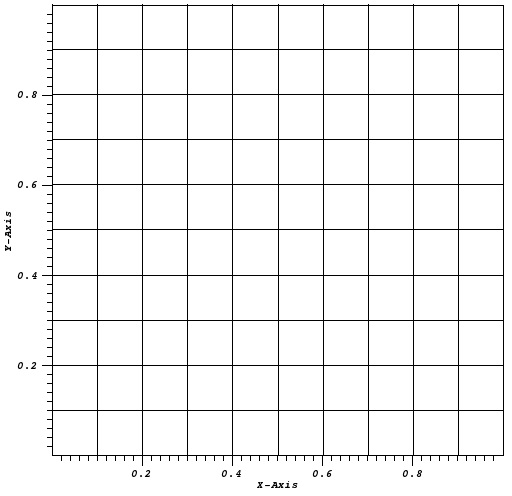
\includegraphics[width=0.82\textwidth]{figures/sec_DSA/SIP_cart_mesh.png}
		\caption{}
	\end{subfigure}
	\vfill
	\begin{subfigure}[b]{0.45\textwidth}
		\centering
		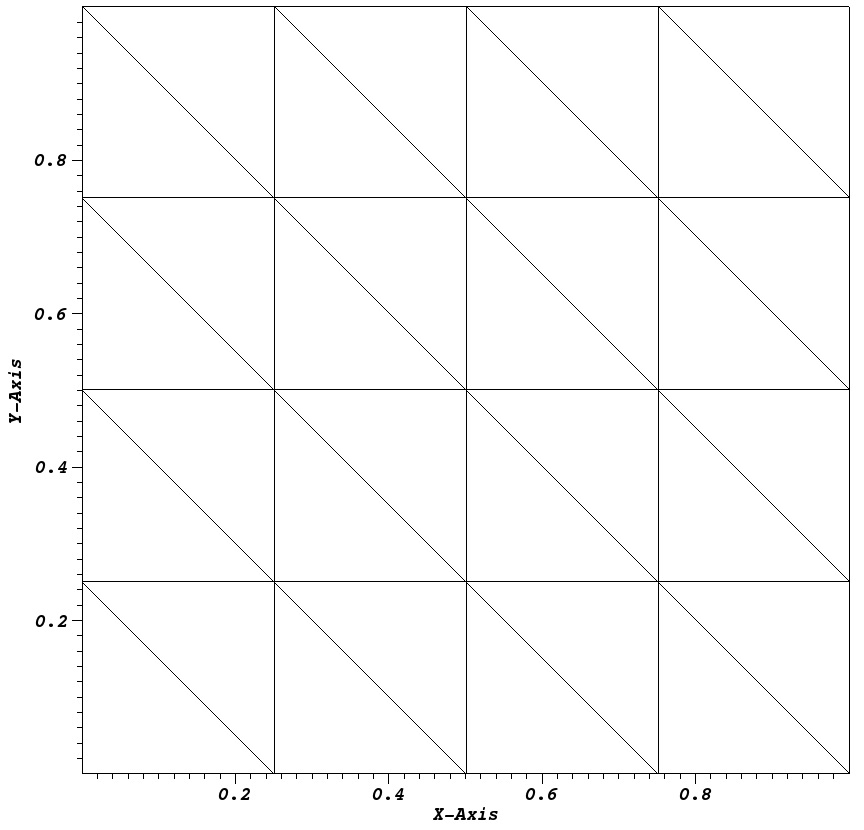
\includegraphics[width=0.85\textwidth]{figures/sec_DSA/SIP_tri_mesh.png}
		\caption{}
	\end{subfigure}
	\hfill
	\begin{subfigure}[b]{0.45\textwidth}
		\centering
		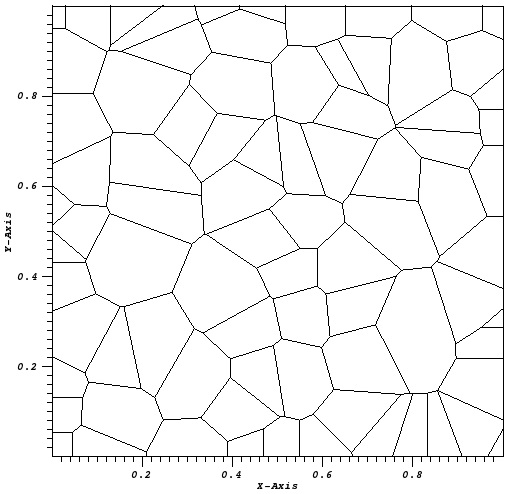
\includegraphics[width=0.85\textwidth]{figures/sec_DSA/SIP_poly_mesh.png}
		\caption{}
	\end{subfigure}
	\vfill
	\begin{subfigure}[b]{0.45\textwidth}
		\centering
		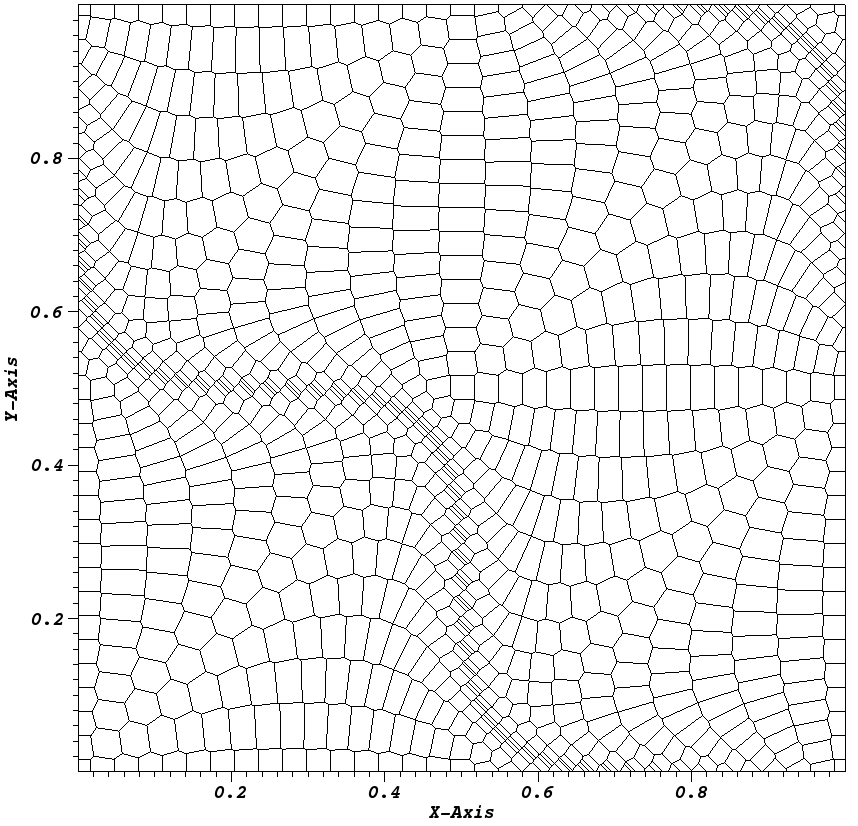
\includegraphics[width=0.85\textwidth]{figures/sec_DSA/SIP_sine_poly_mesh.png}
		\caption{}
	\end{subfigure}
	\hfill
	\begin{subfigure}[b]{0.45\textwidth}
		\centering
		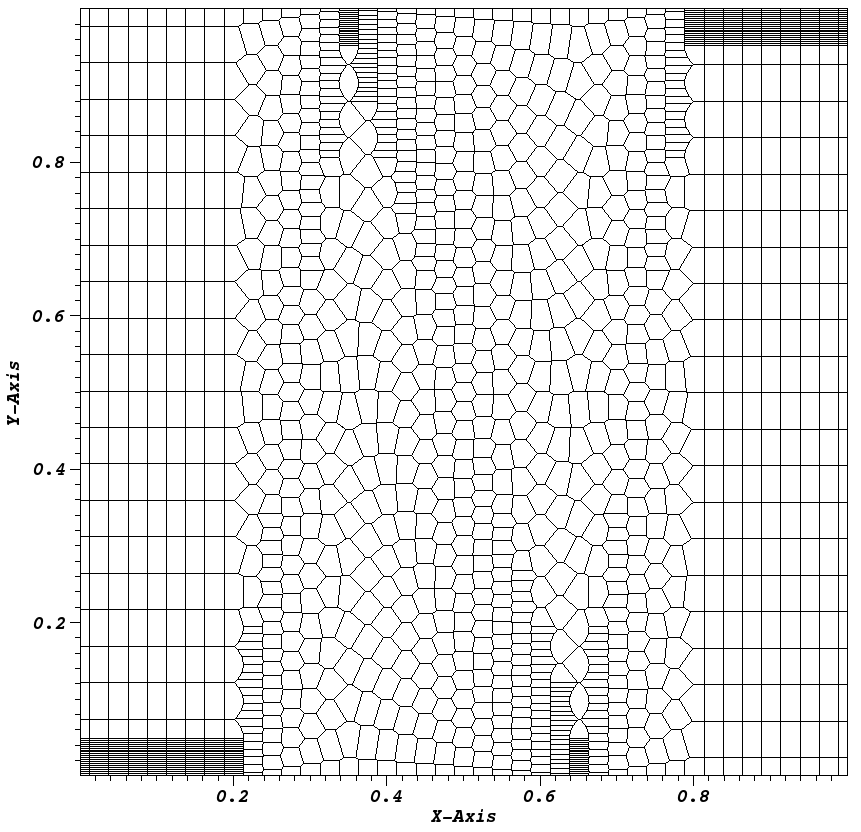
\includegraphics[width=0.85\textwidth]{figures/sec_DSA/SIP_z_poly_mesh.png}
		\caption{}
	\end{subfigure}
\caption{Axial slices of the different mesh types: (a) cartesian, (b) ordered triangles, (c) random polygons, (d) sinusoidal polygons, and (e) polygonal z-mesh.}
\label{fig::SIP_mesh_slices}
\end{figure}

\begin{figure}
\centering
	\begin{subfigure}[b]{0.5\textwidth}
		\centering
		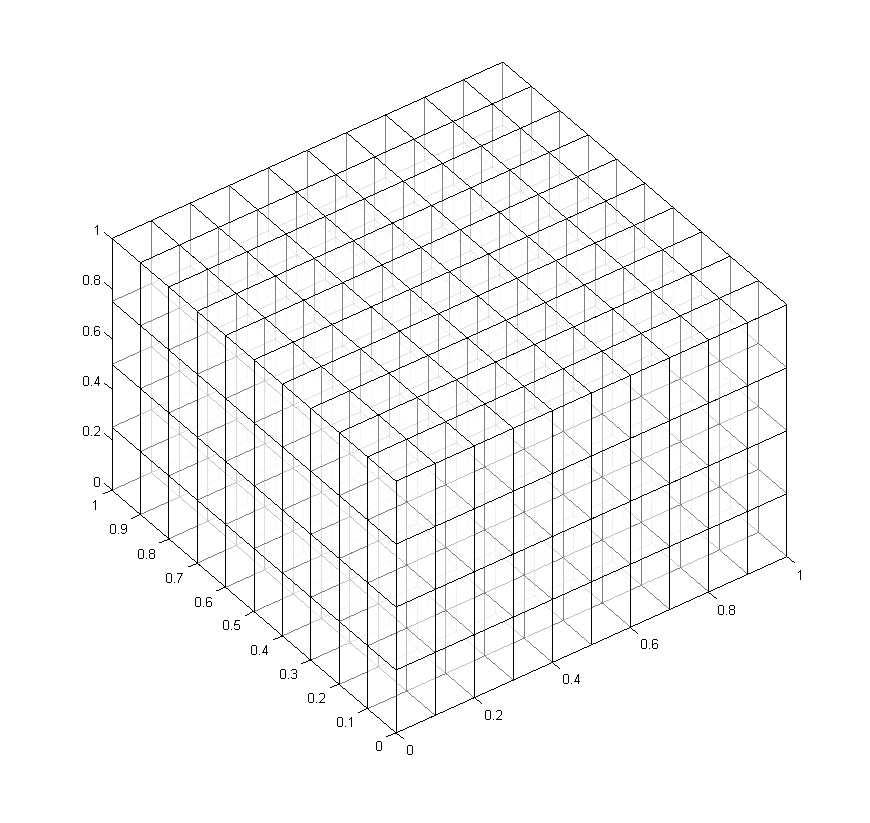
\includegraphics[width=0.82\textwidth]{figures/sec_DSA/SIP_cart_extruded_mesh.png}
		\caption{}
	\end{subfigure}
	\vfill
	\begin{subfigure}[b]{0.45\textwidth}
		\centering
		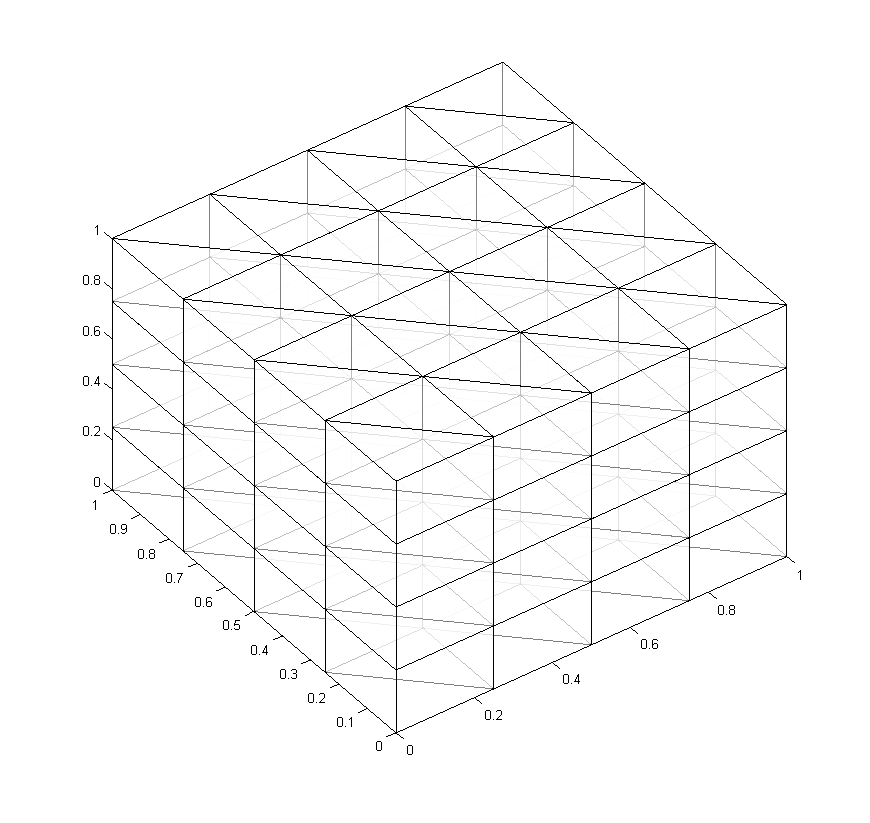
\includegraphics[width=0.85\textwidth]{figures/sec_DSA/SIP_tri_extruded_mesh.png}
		\caption{}
	\end{subfigure}
	\hfill
	\begin{subfigure}[b]{0.45\textwidth}
		\centering
		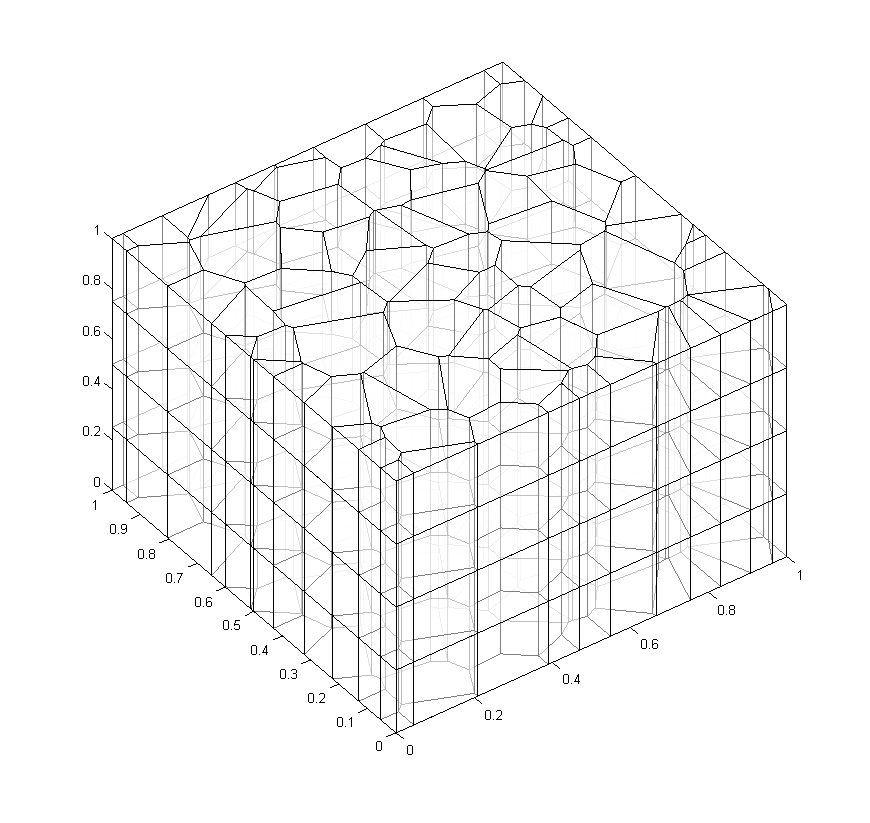
\includegraphics[width=0.85\textwidth]{figures/sec_DSA/SIP_poly_extruded_mesh.png}
		\caption{}
	\end{subfigure}
	\vfill
	\begin{subfigure}[b]{0.45\textwidth}
		\centering
		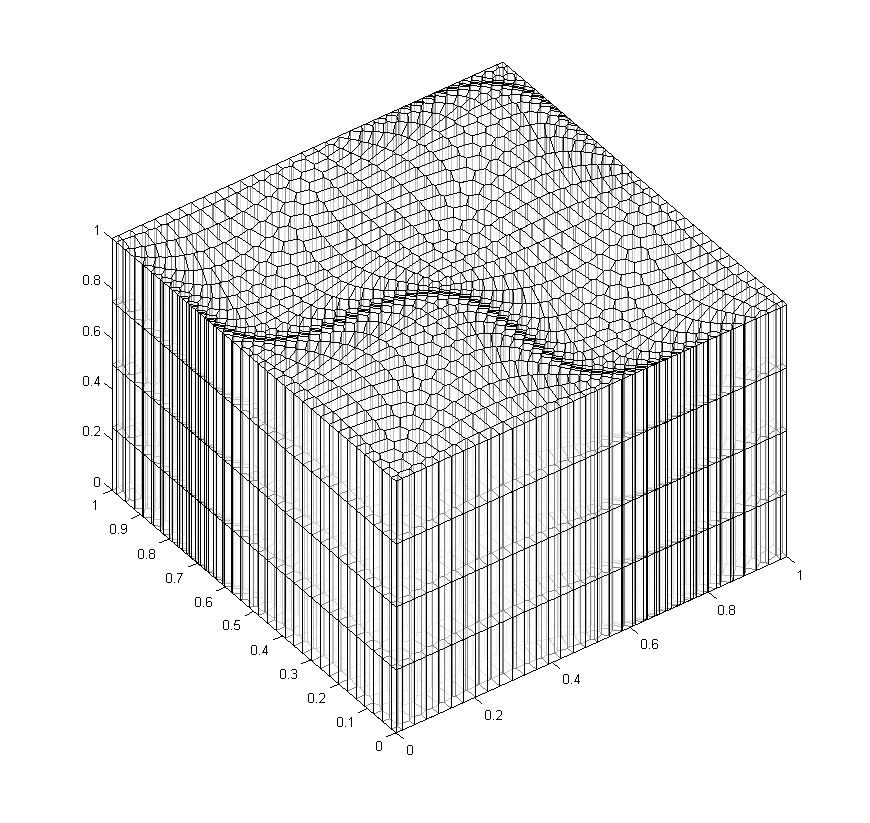
\includegraphics[width=0.85\textwidth]{figures/sec_DSA/SIP_sine_poly_extruded_mesh.png}
		\caption{}
	\end{subfigure}
	\hfill
	\begin{subfigure}[b]{0.45\textwidth}
		\centering
		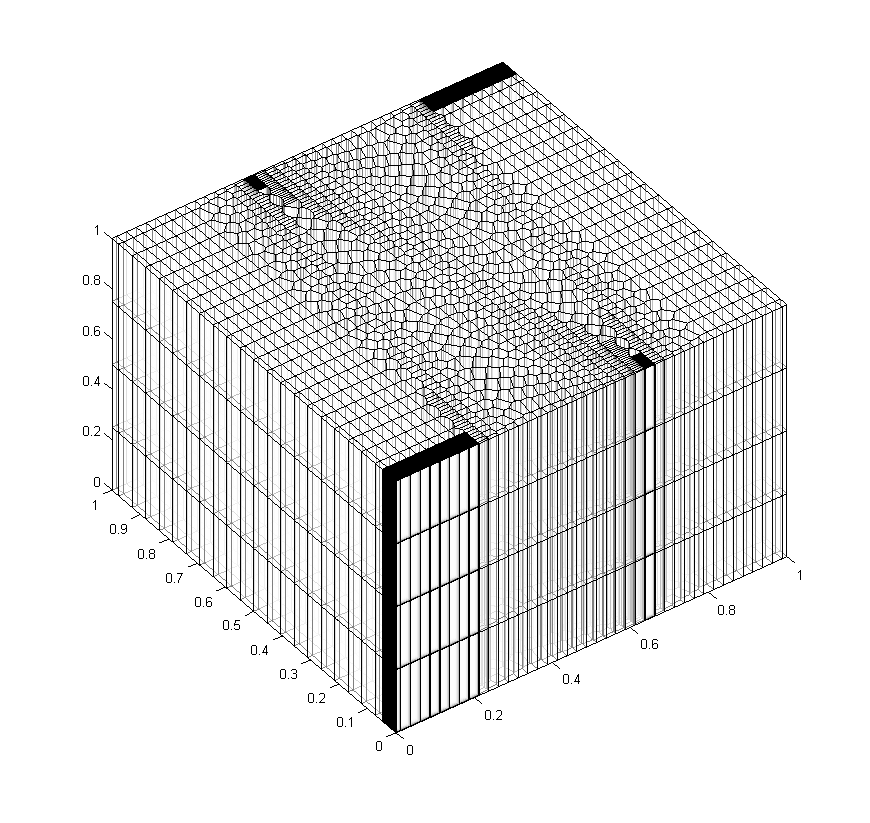
\includegraphics[width=0.85\textwidth]{figures/sec_DSA/SIP_z_poly_extruded_mesh.png}
		\caption{}
	\end{subfigure}
\caption{Extrusion of the different mesh types: (a) cartesian, (b) ordered triangles, (c) random polygons, (d) sinusoidal polygons, and (e) polygonal z-mesh.}
\label{fig::SIP_mesh_extruded}
\end{figure}

%%%%%%%%%%%%%%%%%%%%%%%%%%%%%%%%%%%%%%%%%%%%%%%%%%%
%%%   SubSubSection - SIP Results = Linear
\subsubsection{Purely-Linear Solution}
\label{sec::DSA_Results_SIP_Linear}

We first test SIP by enforcing a sytem that yields a purely-linear solution. Linear finite elements should then theoretically fully-span the solution space. We can achieve this mathematically by setting the cross-section and right-hand-source terms to zero, $\sigma = Q = 0$. Robin boundary conditions are imposed on opposite faces in 1 dimension, with homogeneous Neumann boundary conditions on all other faces. If the Robin boundaries are chosen in the y-direction, with $y \in (0,L)$, then the analytical solution for the problem will be 

\begin{equation}
\label{eq::mms_lin_solution}
\Phi(x,y,z) = \frac{4 J^{inc}}{L + 4D} \left(  L + 2 D - y \right),
\end{equation}

\noindent with the following boundary conditions in the y-direction:

\begin{equation}
\label{eq::mms_lin_bcs}
\begin{aligned}
\Phi - 2D \partial_y \Phi = & 4 J^{inc}, \qquad & \forall (x,z),y=0 \\
\Phi + 2D \partial_y \Phi = & 0, \qquad & \forall (x,z),y=L
\end{aligned}.
\end{equation}

\begin{figure}
\centering
	\begin{subfigure}[b]{0.5\textwidth}
		\centering
		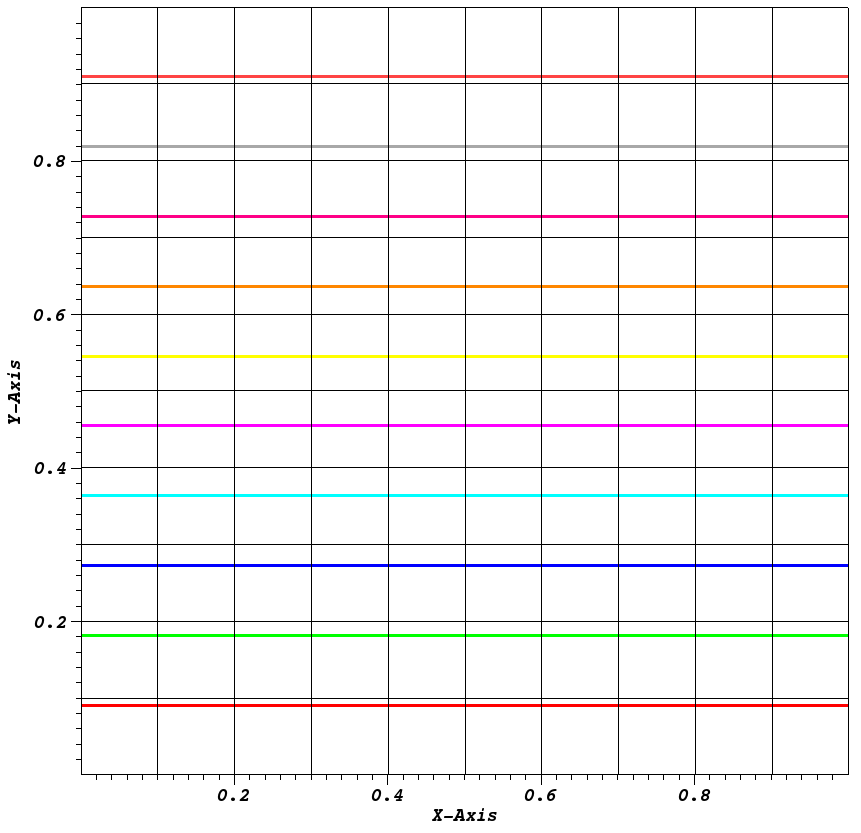
\includegraphics[width=0.82\textwidth]{figures/sec_DSA/SIP_cart_lin_contour.png}
		\caption{}
	\end{subfigure}
	\vfill
	\begin{subfigure}[b]{0.45\textwidth}
		\centering
		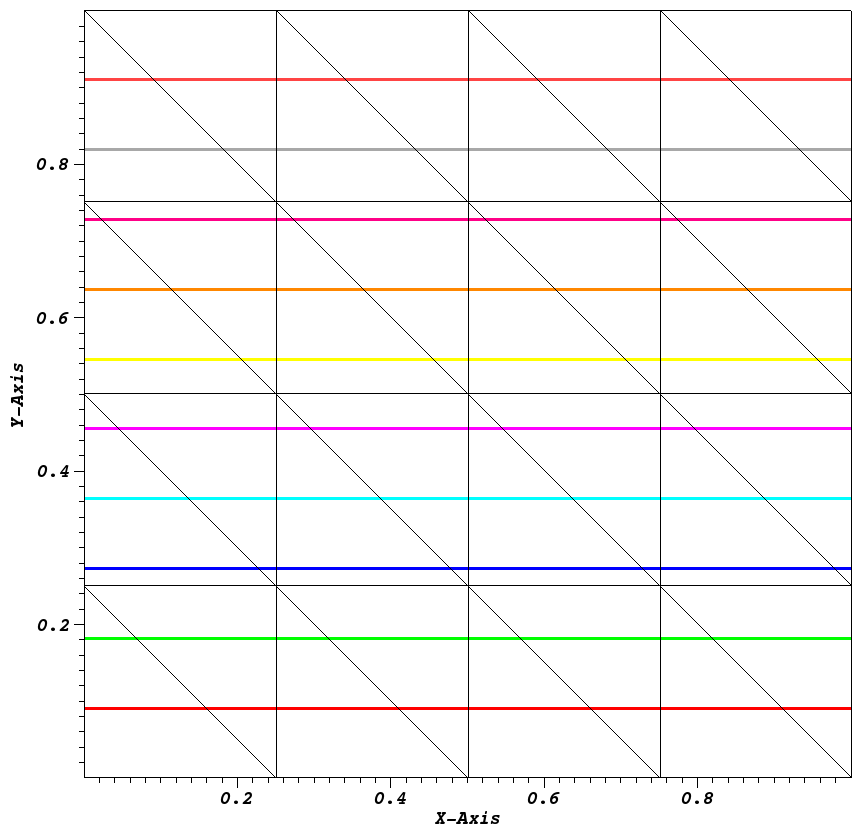
\includegraphics[width=0.85\textwidth]{figures/sec_DSA/SIP_tri_lin_contour.png}
		\caption{}
	\end{subfigure}
	\hfill
	\begin{subfigure}[b]{0.45\textwidth}
		\centering
		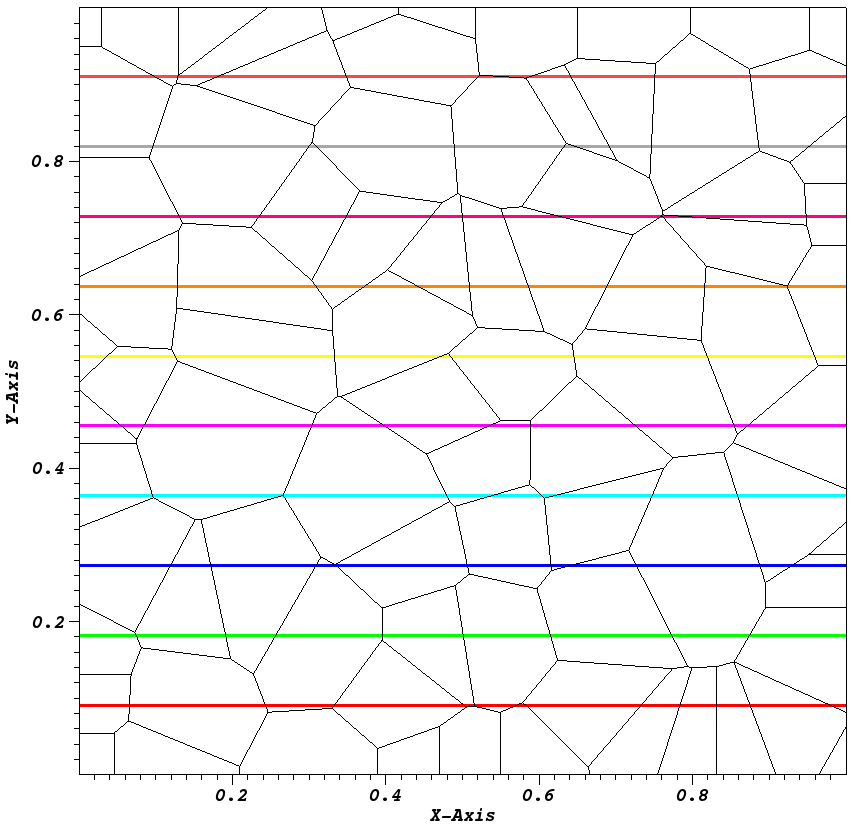
\includegraphics[width=0.85\textwidth]{figures/sec_DSA/SIP_poly_lin_contour.png}
		\caption{}
	\end{subfigure}
	\vfill
	\begin{subfigure}[b]{0.45\textwidth}
		\centering
		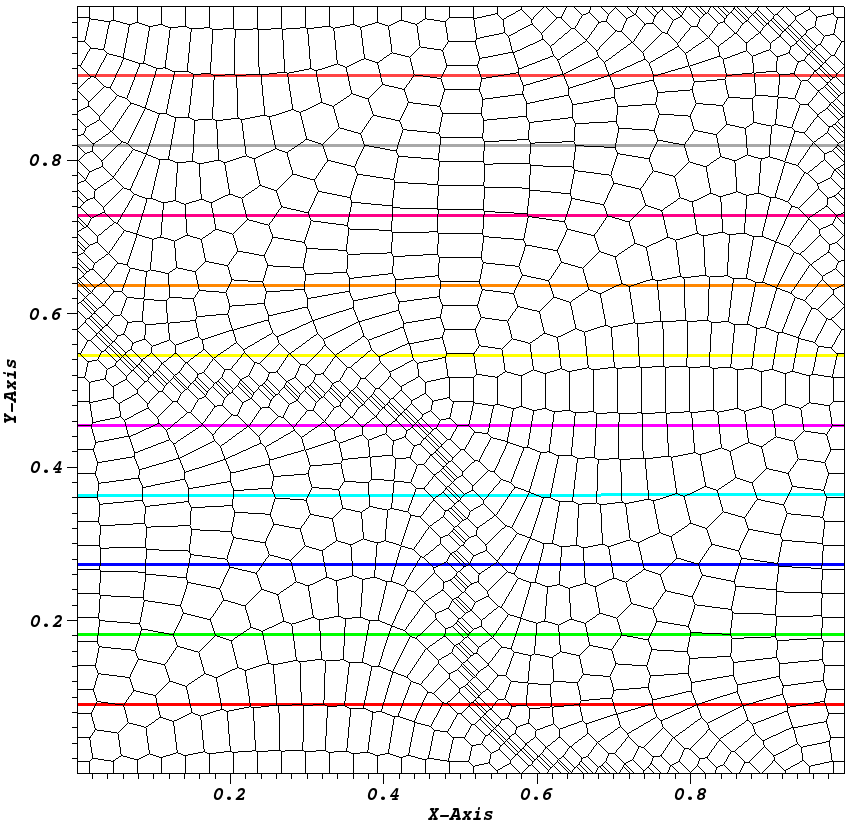
\includegraphics[width=0.85\textwidth]{figures/sec_DSA/SIP_sine_poly_lin_contour.png}
		\caption{}
	\end{subfigure}
	\hfill
	\begin{subfigure}[b]{0.45\textwidth}
		\centering
		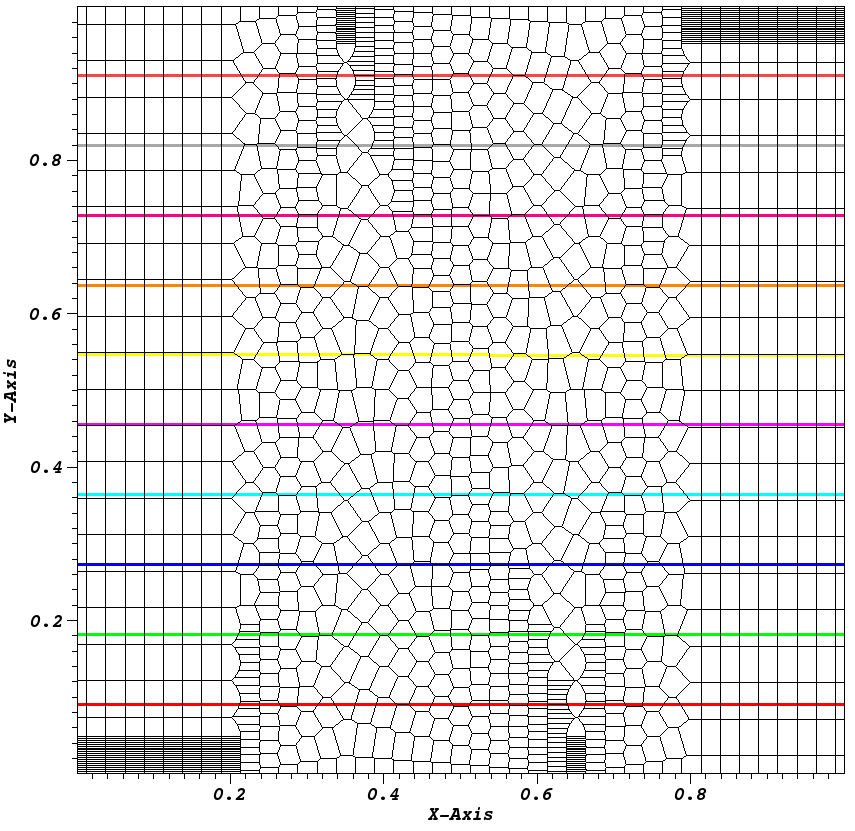
\includegraphics[width=0.85\textwidth]{figures/sec_DSA/SIP_z_poly_lin_contour.png}
		\caption{}
	\end{subfigure}
\caption{Axial slice showing the contours for the linear solution of the different mesh types: (a) cartesian, (b) ordered triangles, (c) random polygons, (d) sinusoidal polygons, and (e) polygonal z-mesh.}
\label{fig::SIP_mesh_slices}
\end{figure}

%%%%%%%%%%%%%%%%%%%%%%%%%%%%%%%%%%%%%%%%%%%%%%%%%%%
%%%   SubSubSection - SIP Results = MMS
\subsubsection{Method of Manufactured Solutions}
\label{sec::DSA_Results_SIP_MMS}

\begin{equation}
\label{eq::SIP_quad_mms_solution}
\begin{aligned}
\Phi^{quad} (x,y,z) = x(1-x)y(1-y)z(1-z) 
\end{aligned}
\end{equation}

\begin{equation}
\label{eq::SIP_gauss_mms_solution}
\begin{aligned}
\Phi^{gauss} (x,y,z) = \Phi^{quad} (x,y,z) \exp(- (\vec{r} - \vec{r}_0) \cdot (\vec{r} - \vec{r}_0)^{T}  )
\end{aligned}
\end{equation}


\begin{figure}
\centering
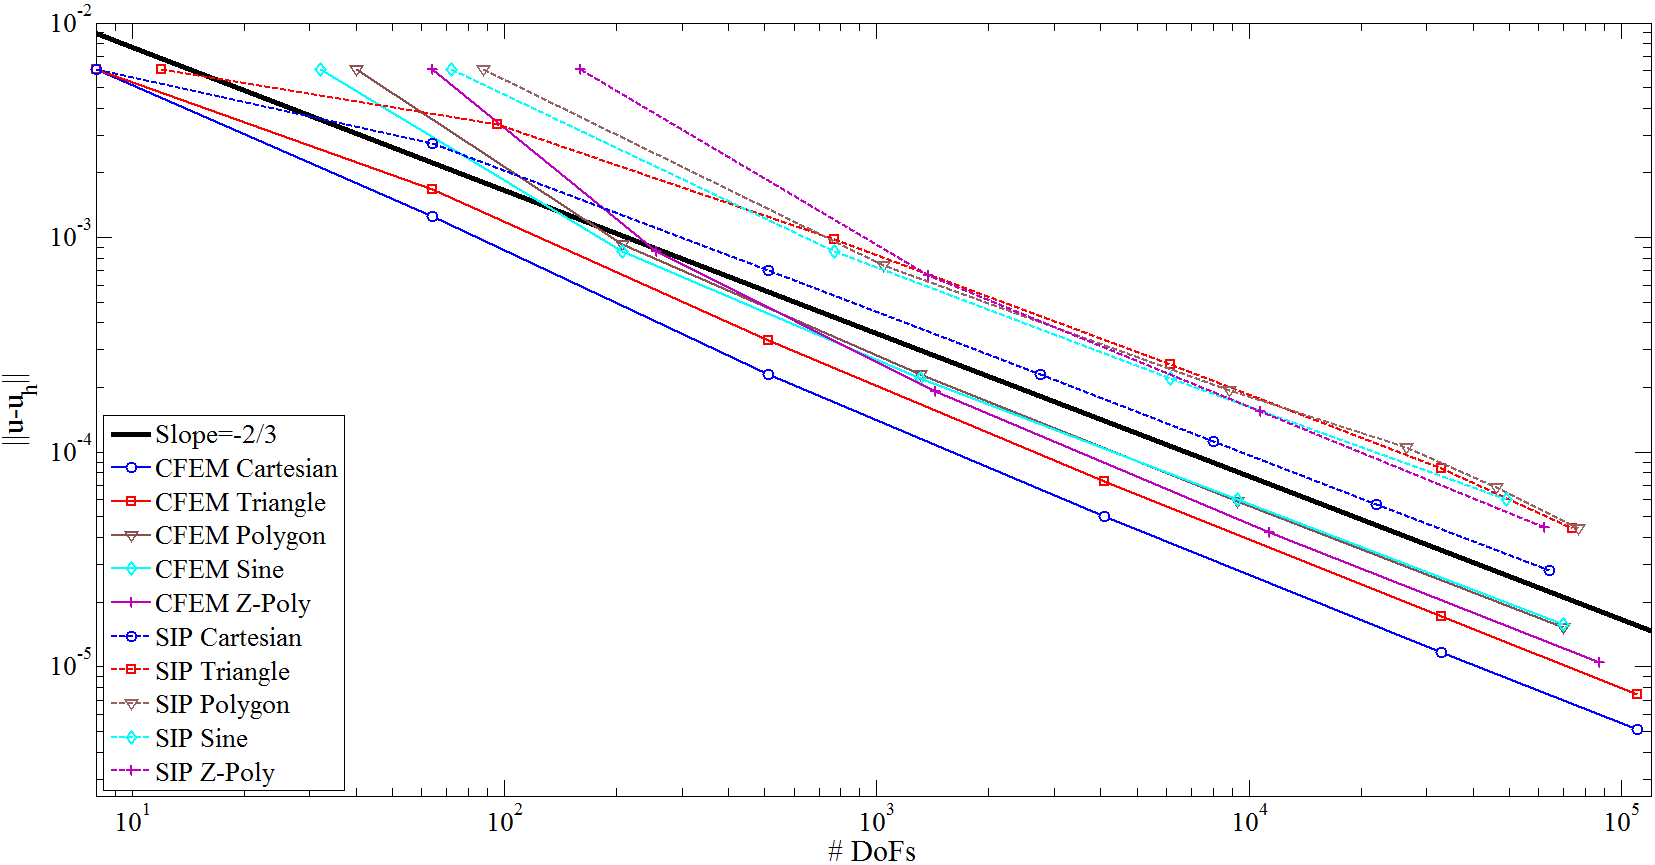
\includegraphics[width=\textwidth]{figures/sec_DSA/SIP_mms_3d_quad_full_paint.png}
\caption{blah}
\label{fig::SIP_mms_quad_error_plot}
\end{figure}

\begin{figure}
\centering
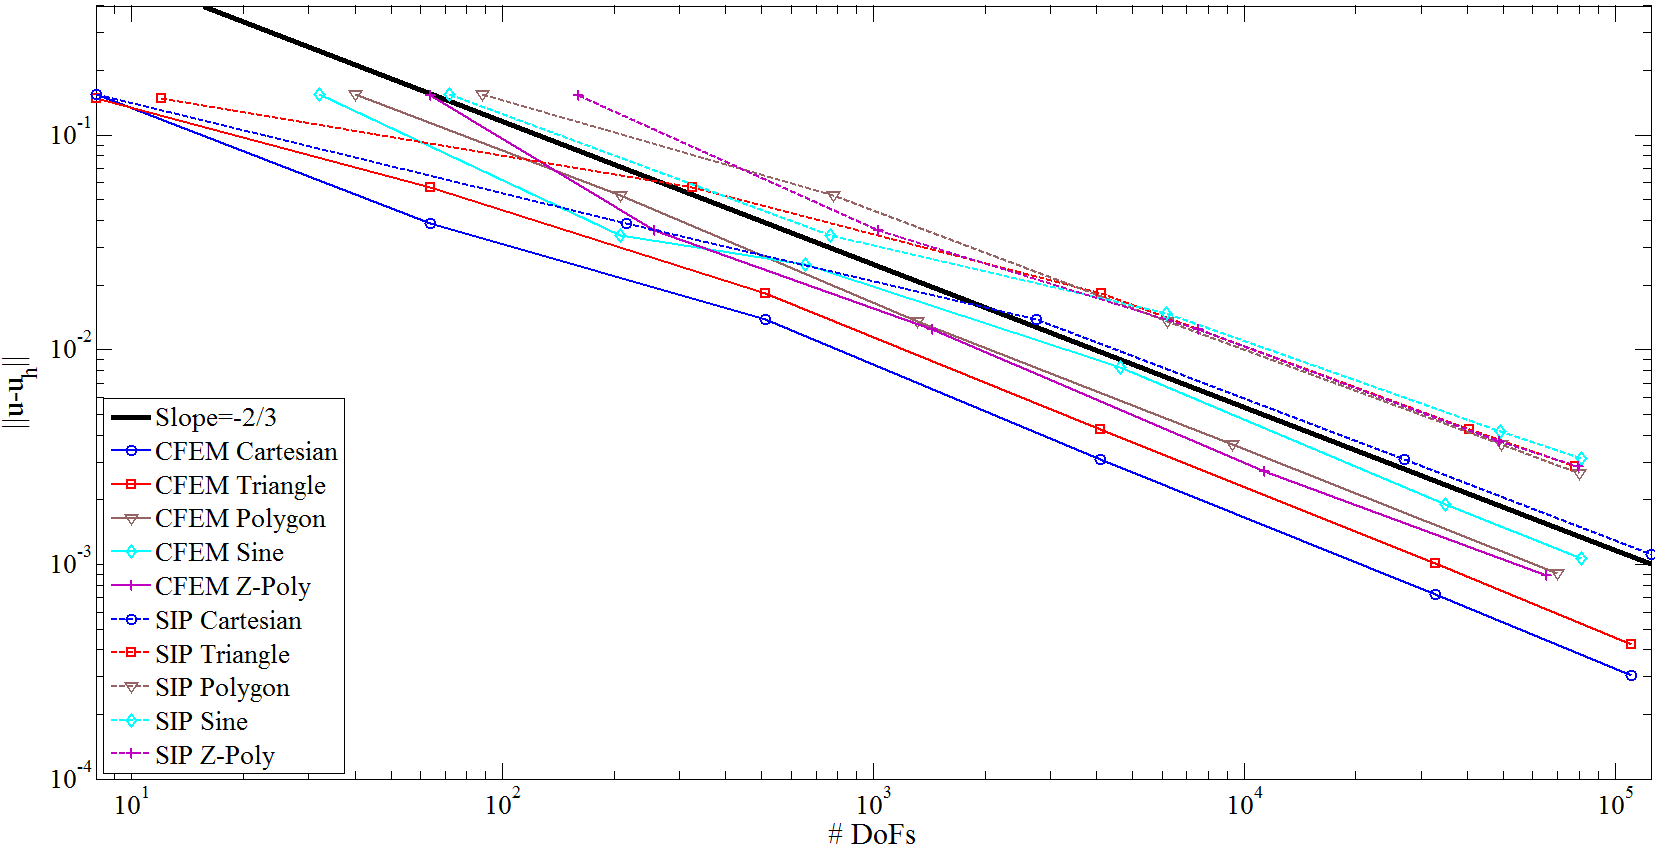
\includegraphics[width=\textwidth]{figures/sec_DSA/SIP_mms_3d_gauss_full_paint.png}
\caption{blah}
\label{fig::SIP_mms_gauss_error_plot}
\end{figure}


%%%%%%%%%%%%%%%%%%%%%%%%%%%%%%%%%%%%%%%%%%%%%%%%%%%
%%%%%%%%%%%%%%%%%%%%%%%%%%%%%%%%%%%%%%%%%%%%%%%%%%%
%%%   SubSection - Fourier Results
\subsection{Fourier Analysis}
\label{sec::DSA_Results_Fourier}

%%%%%%%%%%%%%%%%%%%%%%%%%%%%%%%%%%%%%%%%%%%%%%%%%%%
%%%   SubSubSection - Fourier Results = Homogeneous Medium
\subsubsection{Homogeneous Medium Case}
\label{sec::DSA_Results_Fourier_Homo}

\begin{figure}
\centering
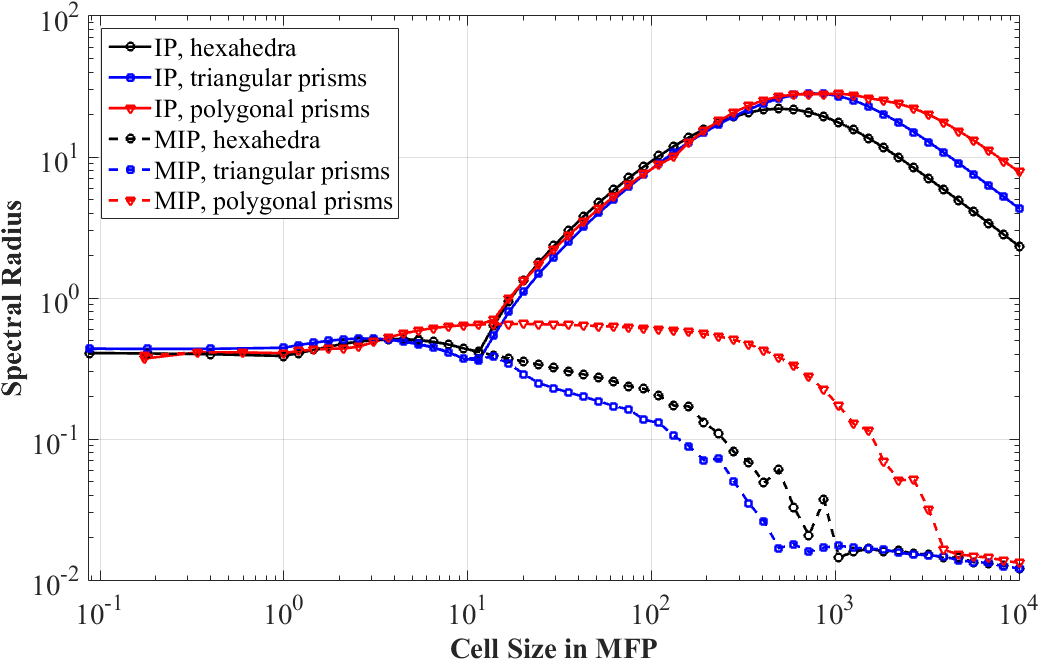
\includegraphics[width=\textwidth]{figures/sec_DSA/IP,MIP_V_hex,tri,poly_LS8_C=4.png}
\caption{blah}
\label{fig::IP_MIP_Homo_LS8_C4}
\end{figure}

%%%%%%%%%%%%%%%%%%%%%%%%%%%%%%%%%%%%%%%%%%%%%%%%%%%
%%%   SubSubSection - Fourier Results = PHI
\subsubsection{Periodic Horizontal Interface (PHI) Problem}
\label{sec::DSA_Results_Fourier_PHI}


%%%%%%%%%%%%%%%%%%%%%%%%%%%%%%%%%%%%%%%%%%%%%%%%%%%
%%%%%%%%%%%%%%%%%%%%%%%%%%%%%%%%%%%%%%%%%%%%%%%%%%%
%%%   SubSection - MIP Results
\subsection{MIP Results}
\label{sec::DSA_Results_MIP}

We have given a theoretical basis for MIP's stability using Fourier Analysis in Section \ref{sec::DSA_Results_Fourier}. In this Section, we provide numerical results of DSA preconditioning of the Discontinuous $S_N$ Transport Equation. We first provide 

%%%%%%%%%%%%%%%%%%%%%%%%%%%%%%%%%%%%%%%%%%%%%%%%%%%
%%%   SubSubSection - MIP Results = Simple Homo Domain
\subsubsection{Simple Homogeneous Problem Results}
\label{sec::DSA_Results_MIP_Homo}

%%%%%%%%%%%%%%%%%%%%%%%%%%%%%%%%%%%%%%%%%%%%%%%%%%%
%%%   SubSubSection - MIP Results = Hetero
\subsubsection{Heterogenous Problem Results}
\label{sec::DSA_Results_MIP_Hetero}


%%%%%%%%%%%%%%%%%%%%%%%%%%%%%%%%%%%%%%%%%%%%%%%%%%%
%%%%%%%%%%%%%%%%%%%%%%%%%%%%%%%%%%%%%%%%%%%%%%%%%%%
%%%   Section - Conclusions
%%%%%%%%%%%%%%%%%%%%%%%%%%%%%%%%%%%%%%%%%%%%%%%%%%%
%%%%%%%%%%%%%%%%%%%%%%%%%%%%%%%%%%%%%%%%%%%%%%%%%%%
\section{Conclusions}
\label{sec::DSA_conclusions}

In this chapter, we have presented a discontinuous form of the diffusion equation, known as the Modified Interior Penalty Method (MIP), which can be applied to the discontinuous finite element form of the transport equation as a DSA preconditioner. 
